\chapter{Command Pattern}

\section{Định nghĩa}
\begin{itemize}
\item Command Pattern là một trong những Pattern thuộc nhóm hành vi (Behavior Pattern). Nó cho phép chuyển yêu cầu thành đối tượng độc lập, có thể được sử dụng để tham số hóa các đối tượng với các yêu cầu khác nhau như log, queue (undo/redo), transtraction. Nói cách khác, Command Pattern cho phép tất cả những request gửi đến object được lưu trữ trong chính object đó dưới dạng một object Command. Khái niệm Command Object giống như một class trung gian được tạo ra để lưu trữ các câu lệnh và trạng thái của object tại một thời điểm nào đó.
\item Command dịch ra nghĩa là ra lệnh. Commander nghĩa là chỉ huy, người này không làm mà chỉ ra lệnh cho người khác làm. Như vậy, phải có người nhận lệnh và thi hành lệnh. Người ra lệnh cần cung cấp một class đóng gói những mệnh lệnh. Người nhận mệnh lệnh cần phân biệt những interface nào để thực hiện đúng mệnh lệnh.
\item Command Pattern còn được biết đến như là Action hoặc Transaction.
\end{itemize}

\section{Mục đích sử dụng}
\begin{itemize}
\item Tham số hóa các đối tượng theo một hành động thực hiện
\item Tạo và thực thi các yêu cầu vào các thời điểm khác nhau
\item Hỗ trợ tính năng undo, log, callback hoặc transaction
\end{itemize}

\section{Command Pattern trong thực tế}

\section{Mô hình cấu trúc}
\begin{center}
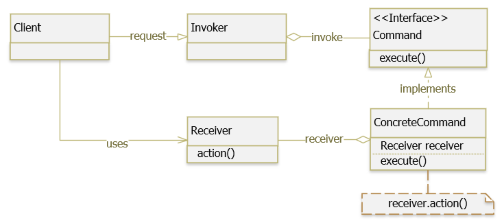
\includegraphics{GALLEYS/images/chapter7/diagram}
\end{center}
Các thành phần:
\begin{itemize}
\item Command : là một interface hoặc abstract class, chứa một phương thức trừu tượng thực thi (execute) một hành động (operation). Request sẽ được đóng gói dưới dạng Command.
\item ConcreteCommand : là các implementation của Command. Định nghĩa một sự gắn kết giữa một đối tượng Receiver và một hành động. Thực thi execute() bằng việc gọi operation đang hoãn trên Receiver. Mỗi một ConcreteCommand sẽ phục vụ cho một case request riêng.
\item Client : tiếp nhận request từ phía người dùng, đóng gói request thành ConcreteCommand thích hợp và thiết lập receiver của nó.
\item Invoker : tiếp nhận ConcreteCommand từ Client và gọi execute() của ConcreteCommand để thực thi request.
\item Receiver : đây là thành phần thực sự xử lý business logic cho case request. Trong phương execute() của ConcreteCommand chúng ta sẽ gọi method thích hợp trong Receiver.
\end{itemize}
Như vậy, Client và Invoker sẽ thực hiện việc tiếp nhận request. Còn việc thực thi request sẽ do Command, ConcreteCommand và Receiver đảm nhận.
